
%%%%%%%%%%%%%%%%%%%%%%%%%%%%%%%%%%%%%%%%%%%%%%%%%%%%%%%%%%%%%%%%%%%%%%%%%%%%%
\section{Code tests}
\label{sec.tests}

%%%%%%%%%%%%%%%%%%%%%%%%%%%%%%%%%%%%%%%%%%%%%%%%%%%%%%%%%%%%%%%%%%%%%%%%%%%%%
\subsection{Verifying and validating the \enzo\ code}
\label{sec.tests.vandv}

\red{(Britton)} Description of test suite and test runner.

\red{(Brian)} Refer to all code comparisons that Enzo has been part of.

%%%%%%%%%%%%%%%%%%%%%%%%%%%%%%%%%%%%%%%%%%%%%%%%%%%%%%%%%%%%%%%%%%%%%%%%%%%%%
\subsection{Representative test problems}
\label{sec.tests.problems}

General structure for each test problem:  Outline how the test problem is constructed (initial and boundary conditions), 
the analytical solution, why we have in the paper (what does it break, or what flaw does it expose (not in enzo of course)),
a plot showing how well enzo solves said test problem, and a brief description of the plot and how awesome enzo is.

%%%%%%%%%%%%%%%%%%%%%%%%%%%%%%%%%%%%%%%
\subsubsection{Sod Shock Tube}
\label{sec.tests.sodshock}
\red{(Greg)}
Problem type 1.  AMR version.  Tests the hydro.
This is also problem 7.2 in the FLASH method paper.

%%%%%%%%%%%%%%%%%%%%%%%%%%%%%%%%%%%%%%%
\subsubsection{Wave pool}
\label{sec.tests.wavepool}
\red{(Greg)}
Problem type 2, with AMR.  Tests reflections of waves at grid boundaries.

%%%%%%%%%%%%%%%%%%%%%%%%%%%%%%%%%%%%%%%
\subsubsection{Shock pool}
\label{sec.tests.shockpool}
\red{(Greg)}
Problem type 3, with AMR.  Tests passage of shock through a refinement boundary.

%%%%%%%%%%%%%%%%%%%%%%%%%%%%%%%%%%%%%%%
\subsubsection{Double mach reflection}
\label{sec.tests.doublemach}
\red{(Brian)}
Problem type 4.  This is one of Alexei's test problems.  Tests
boundary conditions in hydro.

%%%%%%%%%%%%%%%%%%%%%%%%%%%%%%%%%%%%%%%
\subsubsection{Sedov Explosion}
\label{sec.tests.sedov}
\red{(Elizabeth)}

\begin{figure}
\begin{center}
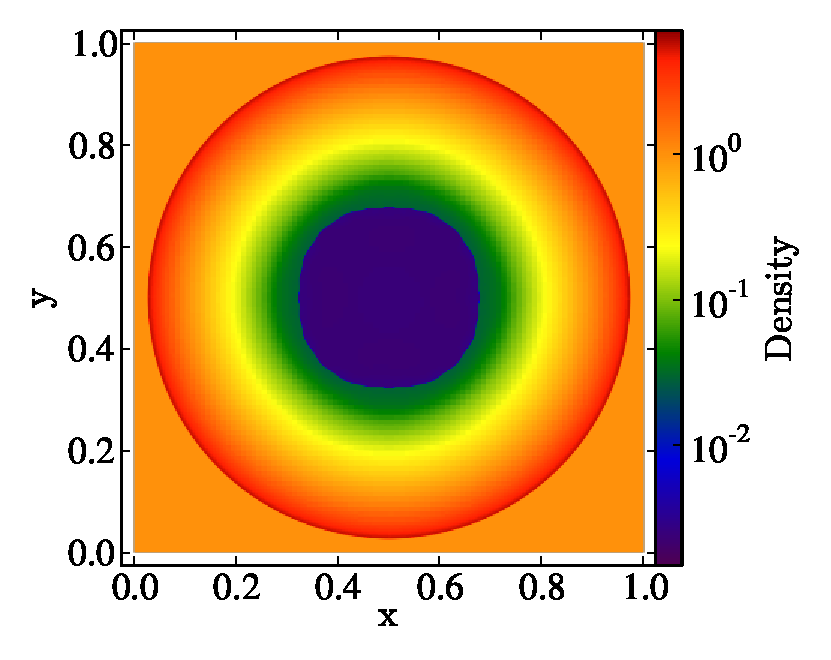
\includegraphics[width=0.4\textwidth]{figures/sedov-ppm-slice.eps}
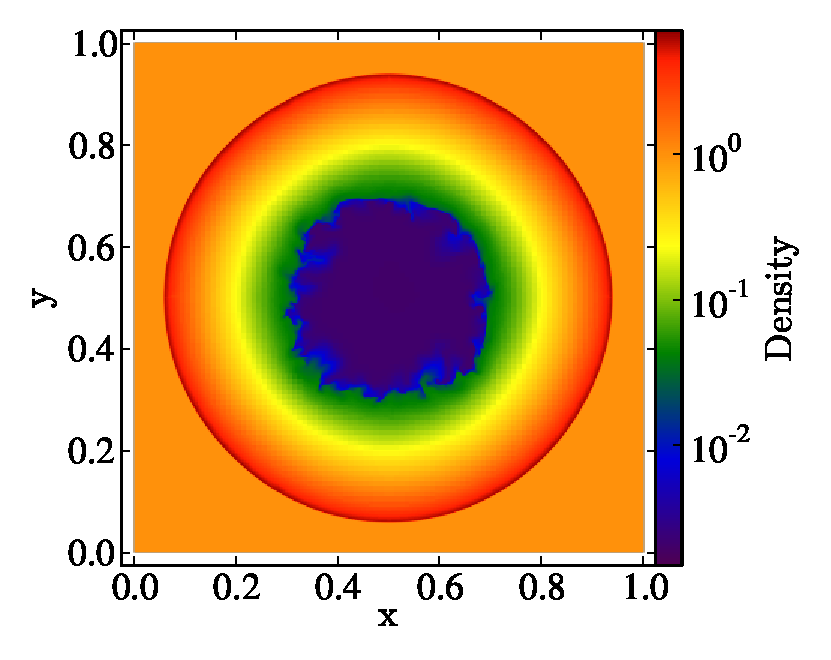
\includegraphics[width=0.4\textwidth]{figures/sedov-zeus-slice.eps}
\caption{Density slice from the Sedov Blast Test at $t = 0.07$. Left-hand image shows the results from PPM ({\tt HydroMethod = 0}), right-hand image shows the results from Zeus ({\tt Hydromethod = 2}). Notably, the Zeus shock front has progressed less far than forthe PPM run. This is due to energy loss when conserving internal, not total, energy.}
\label{fig.sedov1}
\end{center}
\end{figure}


\begin{figure}
\begin{center}
\includegraphics[width=\textwidth]{figures/sedov-profiles.eps}
\caption{Radially averaged profiles for the Sedov Blast Test at $t = 0.07$. Clockwise from top-left shows density, velocity, internal energy and pressure.}
\label{fig.sedov2}
\end{center}
\end{figure}

The Sedov Blast Test \citep{Sedov1959} models an intense explosion, initiated by depositing thermal energy into a homogenous distribution of gas. The result is a strong spherical shock wave centered on the point of energy injection.  This problem is a popular test of astrophysical numerical codes for three reasons: Firstly, it is particularly appropriate to astrophysics since it represents the situation when a supernovae explosion occurs. Secondly, it has an exact analytical solution whereby the shock front's radial position is given by:

\begin{equation}
r(t) = \left(\frac{E_0}{\alpha\rho_0}\right)^{1/5}t^{2/5}
\end{equation}

\noindent where $E_0$ is the initial energy injection, $\rho_0$ is the background density and $\alpha = 1.0$ for cylindrical symmetry and an ideal gas with $\gamma = 1.4$. For the full derivation see \citet{Sedov1959}. This solution makes it possible to assess how well the code performs. Thirdly, the spherical shock is a challenging problem for numerical codes (both grid and particle) since the shock wave increases in size as the simulation progresses and its symmetrical nature highlights any directional preferences that grid codes can succumb to. The test presented here is the two-dimensional version that is included in the Enzo distribution. The three-dimensional results from this test, both for Enzo and three other leading astrophysics codes, can be founds in \citet{Tasker2008}.

In the initial state, the box contains a homogenous distribution of gas at a density of 1 (note that, in the absense of gravity, this problem is scale-free and so without units). Thermal energy is deposited into a single cell at the center of the box with $E_0 = 10.0$. The problem is completed in two dimensions with reflecting boundary conditions (the default for Enzo) and uses a boxsize of side $1$. For this problem, we selected a top grid of $100 \times 100$ and four levels of refinement, placed based on shock location and the slope in density and total energy (this corresponds to cell flagging methods 1 and 3 in the Enzo parameter file). The exception to this scheme is in the initial conditions where grids are placed directly around the injection point. The results were assessed at $t = 0.07$, which corresponding to a time just before the shock reaches the box edge (see Figure~\ref{fig.sedov1}).

Figure~\ref{fig.sedov2} shows the radial profiles for the simulation run with the PPM hydro-solver (blue dashed line) and the Zeus hydro-solver (red dash-dot-dot line) together with the analytical solution (black solid line). Clockwise from the top-left are density, velocity, internal energy and pressure. PPM matches the analytical solution extremely well for all quantities. However, Zeus' shock front lags behind the analytical position. This can also be seen in the slices shown in Figure~\ref{fig.sedov1}. The cause of this discrepancy is that Zeus shows a substantial energy lost during the first few timesteps and produces a diamond-shaped, rather than spherical, shockfront during this time. After this, the code correctly conserves energy but this intial energy loss remains clearly visible in the position of the shock at $t = 0.07$. This problem was addressed directly by \citet{Clarke2010}, who attributed the source of the issue to this version of Zeus solving the internal, rather than total, energy equation. In situations with strong energy gradients, this choice caused an energy loss and the artificial viscosity produces the direction-dependent shockfront shape. In their paper, \citet{Clarke2010} presents results from an alternative version of Zeus that conserves total energy. This problem is less marked for smaller energy gradients and it should be noted that Zeus' stability and speed make it a highly competitive choice, despite the disagreements in this test. 


%%%%%%%%%%%%%%%%%%%%%%%%%%%%%%%%%%%%%%%
\subsubsection{Point source gravity test}
\label{sec.test.gravitypointsource}
\red{(Greg)}
This is the TestGravity (problem 23) test problem.  It tests gravity around a point source, using fixed AMR.

%%%%%%%%%%%%%%%%%%%%%%%%%%%%%%%%%%%%%%%
\subsubsection{Orbit Test}
\label{sec.test.testorbit}
\red{(Greg)}
This is the TestOrbit problem (problem 29 for GB).  This tests gravity and particle integration (no hydro).

%%%%%%%%%%%%%%%%%%%%%%%%%%%%%%%%%%%%%%%
\subsubsection{Self-Similar infall test}
\label{sec.tests.infall}
\red{(Greg)}
Problem type 24.  This is a test based on Bertschinger's 1985 3D self-similar infall
solution, and tests gravity + hydro.

%%%%%%%%%%%%%%%%%%%%%%%%%%%%%%%%%%%%%%%
\subsubsection{Zel`Dovich Pancake}
\label{sec.tests.pancake}
\red{(Brian)}
Problem type 20, unigrid and AMR both.  Tests gravity + hydro.

%%%%%%%%%%%%%%%%%%%%%%%%%%%%%%%%%%%%%%%
\subsubsection{Cosmology simulations}
\label{sec.tests.}
\red{(Brian)}
Talk about cosmology code comparisons, where Enzo is good/weak.

%%%%%%%%%%%%%%%%%%%%%%%%%%%%%%%%%%%%%%%
\subsubsection{MHD: Orszag-Tang Vortex}
\label{sec.tests.mhd}
Figure \ref{fig.orszag} shows the Orszag-Tang vortex problem, a typical test
problem for MHD \citep{Orszag79}.  The left panel shows the MHD-CT result, while
the right panel shows the Dedner result.  This test shows that small scale structure
can be generated in MHD from large scale initial perturbations.  
The test begins 
with uniform density, $\rho_0=25/36 \pi$ and pressure, $P_0=5/12 \pi$.  There is
a single rotational mode in the velocity, and two in the magnetic field: 
${\bf v}_0 $ = (-sin(2$\pi$ y) $ \hat{x}$ , sin(2$\pi$ x) $\hat{y}$),
${\bf B}_0$  =  (-sin(2 $\pi$ y) $ \hat{x},$ sin( 4 $\pi$ x )$\hat{y}$).  The
simulation is evolved to t=0.48.  One can see that the structures are accurately
represented as compared to, for instance, \citet{Toth00}, and that the
resolution of shocks is comparable in both methods.  

{\emph Dave's note:  I'll probably play around with these results in future
versions.}

\begin{figure}
\begin{center}
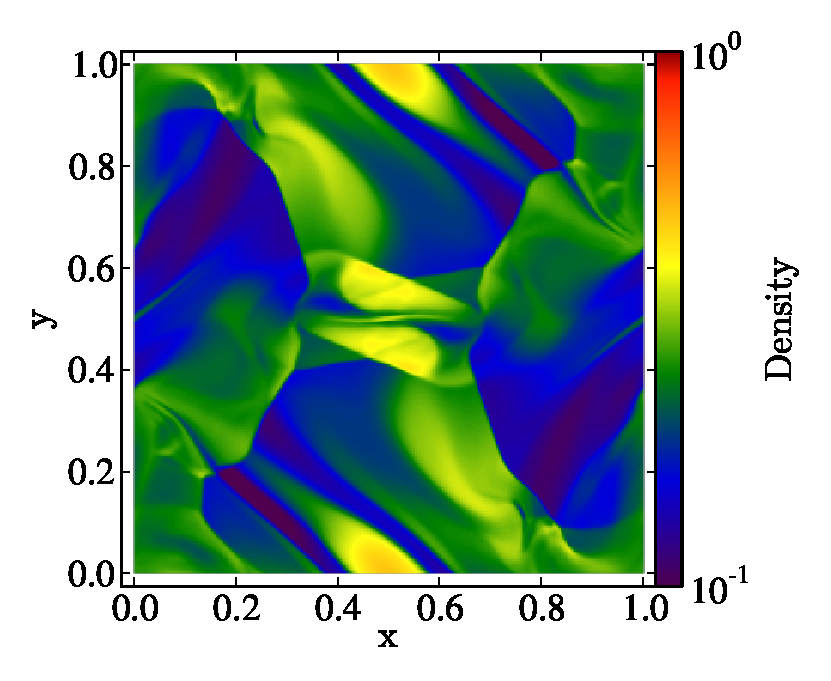
\includegraphics[width=0.4\textwidth]{figures/MHDCT_OrszagTang_Density.eps}
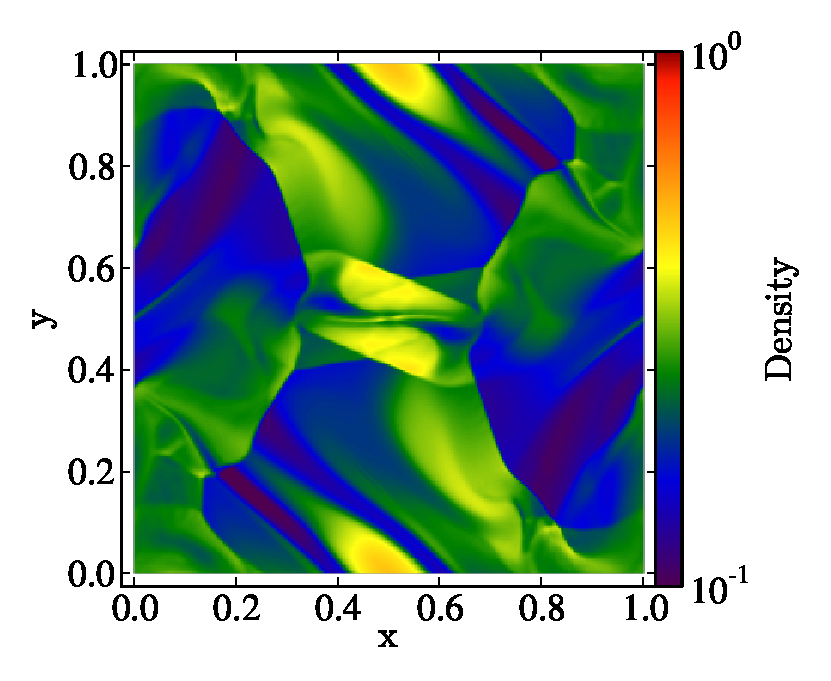
\includegraphics[width=0.4\textwidth]{figures/MHDDedner_OrszagTang_Density.eps}
\caption{TANG}
\label{fig.orszag}
\end{center}
\end{figure}


%%%%%%%%%%%%%%%%%%%%%%%%%%%%%%%%%%%%%%%
\subsubsection{1-zone free-fall test}
\label{sec.tests.freefall}
\red{(Britton)}
One zone free fall test.  Tests cooling, chemistry.

%%%%%%%%%%%%%%%%%%%%%%%%%%%%%%%%%%%%%%%
\subsubsection{Photo-evaporation of a dense clump}
\label{sec.tests.raytracing}
\red{(John)}
Photo-evaporation of a dense clump.  Tests ray tracing, specifically
the shadowing effects of the clump, and the hydrodynamic response of
the clump.

%%%%%%%%%%%%%%%%%%%%%%%%%%%%%%%%%%%%%%%
\subsubsection{Representative FLD test}
\label{sec.tests.fld}

\red{(Dan)}
One test for the implicit FLD: best/hardest one.



%%%%%%%%%%%%%%%%%%%%%%%%%%%%%%%%%%%%%%%

\subsubsection{Representative thermal conduction test}
\label{sec.tests.conduct}
\red{(Brian)}
One test for the thermal conduction (maybe 1 for isotropic, 1 for
anisotropic).
